\section{Appendix: pseudocode and flowcharts} \label{section: appendix}
This appendix provides the full blocks of pseudocode and its flowcharts.

{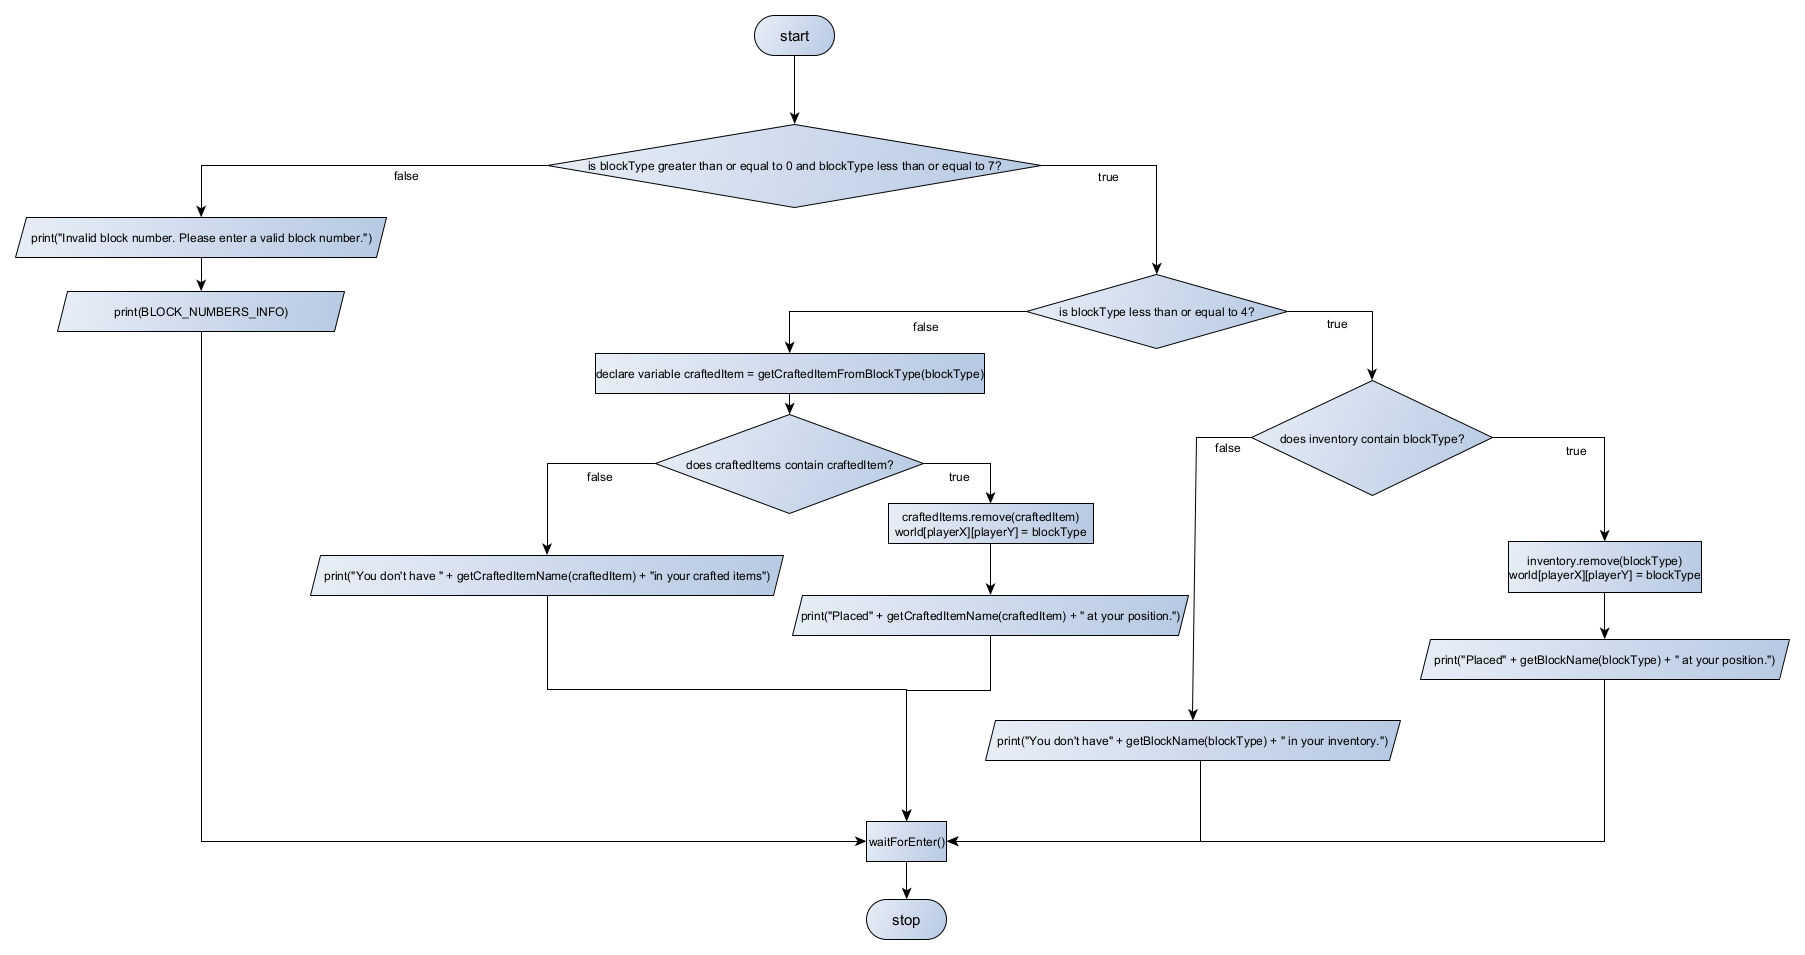
\includegraphics[width=\textwidth]{../flowchart/placeBlock.png}}

\begin{lstlisting}
function placeBlock(blockType)

if blockType is greater than or equal to 0 and blockType is less than or equal to 7 then 
	if blockType less than or equal to 4 then
		if inventory contains blockType then
			inventory.remove(blockType)
			world[playerX][playerY] = blockType
			print("Placed" + getBlockName(blockType) + " at your position.")

		else print("You don't have " + getBlockName(blockType) + " in your inventory")
		end if
	else
		craftedItem = getCraftedItemFromBlockType(blockType)
		if craftedItems contains craftedItem then 
			craftedItems.remove(craftedItem)
			world[playerX][playerY] = blockType
			print("Placed" + getCraftedItemName(craftedItem)+ " at your position.")
		else print("You don't have " + getCraftedItemName() + " in your inventory.")
		end if
	end if
else print("Invalid block number. Please enter a valid block number.")
print(BLOCK_NUMBERS_INFO)
end if
waitForEnter()
end function
\end{lstlisting}
\newpage

{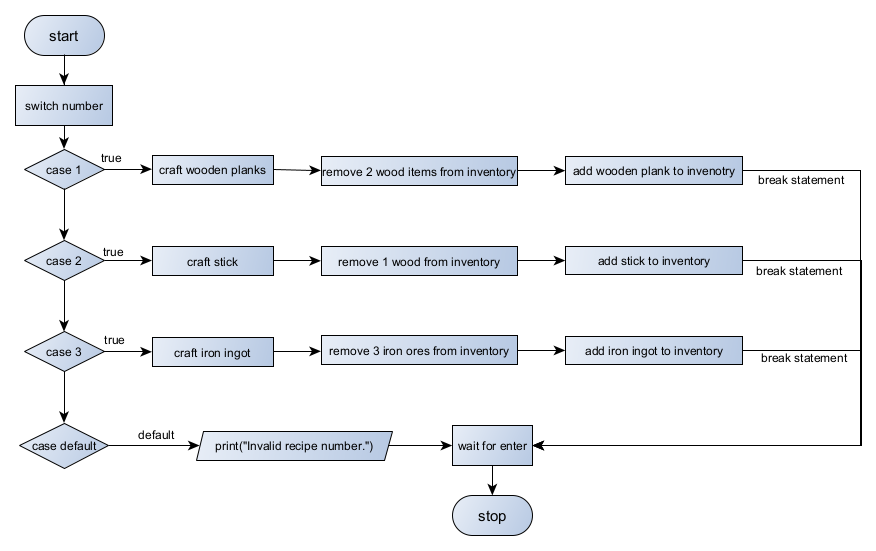
\includegraphics[width=\textwidth]{../flowchart/craftItem.png}}
\begin{lstlisting}
function craftItem(recipe)

switch(recipe)
case 1: 
	craftWoodenPlanks()
end if
case2: 
	craftStick()
end if
case3:
	craftIronIngot()
end if
default: 
	print("Invalid recipe number.")
end switch
waitForEnter()
end function
\end{lstlisting}
\newpage

{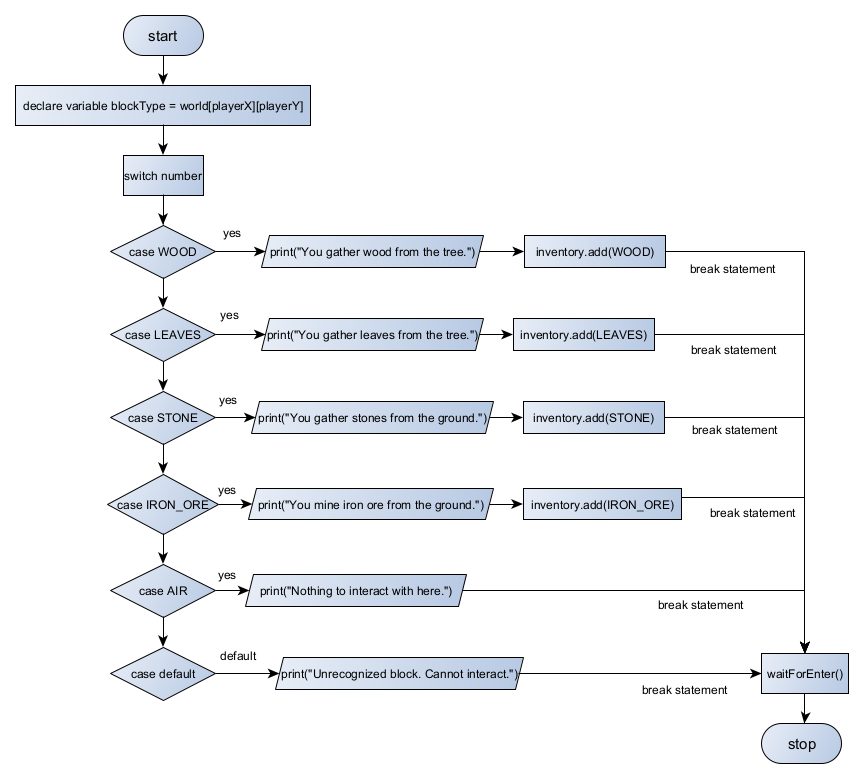
\includegraphics[width=\textwidth]{../flowchart/interactWithWorld.png}}


\begin{lstlisting}
function interactWithWorld()

blockType = world[playerX][playerY]
switch(blockType):
case WOOD: 
	print("You gather wood from the tree.")
	inventory.add(WOOD)
end if
case LEAVES:
	print("You gather leaves from the tree.")
	inventory.add(LEAVES)
end if
case STONE:
	print("You gather stones from the ground.")
	inventory.add(STONE)
end if
case IRON_ORE:
	print("You mine iron ore from the ground.")
	inventory.add(IRON_ORE)
end if
case AIR:
	print("Nothing to interact with here.")
end if
default: print("Unrecognized block. Cannot interact.")
end switch
waitForEnter()
end function
\end{lstlisting}
\newpage

{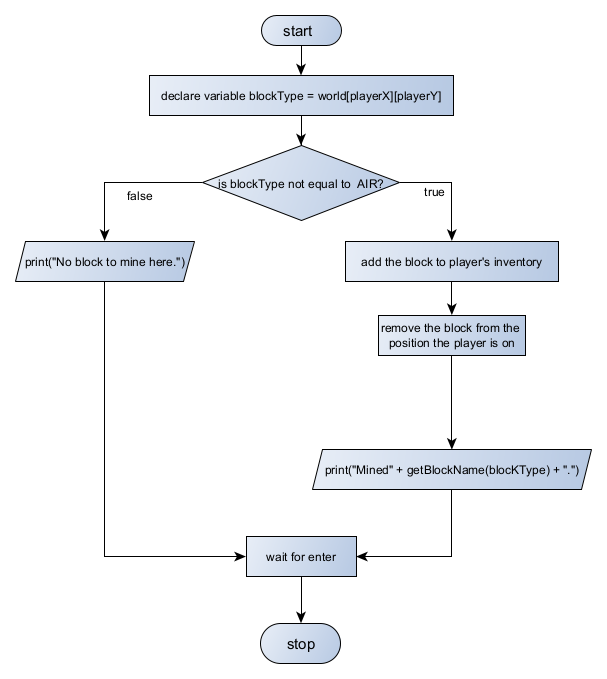
\includegraphics[width=\textwidth]{../flowchart/mineBlock.png}}
\begin{lstlisting}
function mineBlock()

blockType = world[playerX][playerY]
if blockType is not equal to AIR then 
	inventory.add(blockType)
	world[playerX][playerY] = AIR
	print("Mined " + getBlockName(blockType) + ".")
else print("No block to mine here.")
end if
waitForEnter()
end function
\end{lstlisting}
\newpage
{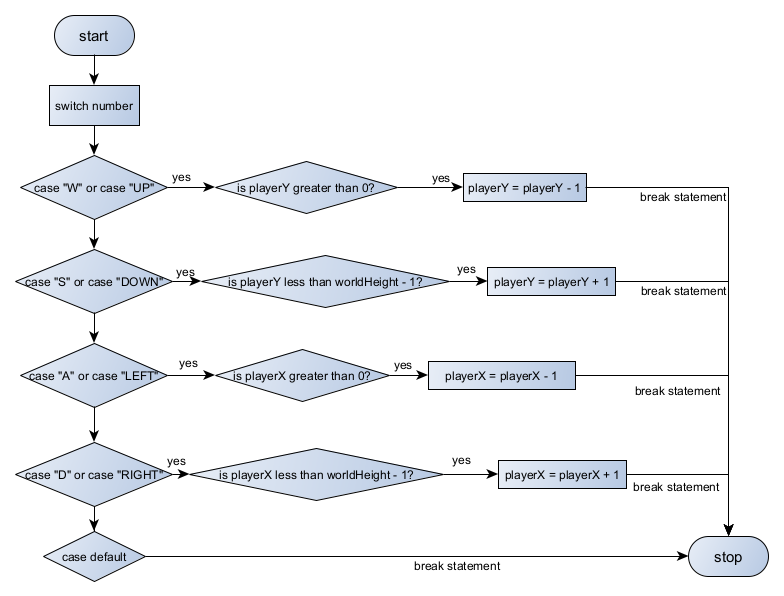
\includegraphics[width=\textwidth]{../flowchart/movePlayer.png}}
\begin{lstlisting}
function movePlayer(direction):

direction = uppercase(direction) //converts direction to uppercase for consistency
switch(direction):
case "W" or "UP":
	if playerY > 0 then playerY = playerY - 1
	end if
case "S" or "DOWN":
	if playerY < worldHeight - 1 then playerY = playerY + 1
	end if
case "A" or "LEFT":
	if playerX > 0 then playerX = playerX - 1
	end if
case "D" or "RIGHT":
	if playerX < worldWidth - 1 then playerX = playerX + 1
	end if
default: //do nothing
end switch
end function
\end{lstlisting}
\newpage

{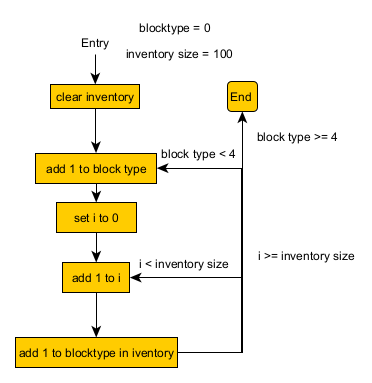
\includegraphics[width=\textwidth]{../flowchart/fillInventory.png}}
\begin{lstlisting}
fillInventory()
Set INVENTORY_SIZE = 100

Clear inventory
FOR blockType = 0; blockType <= 4; blockType ++:
   FOR i = 0; i < INVENTORY_SIZE; i++:
      add block blockType to inventory
      
end function
\end{lstlisting}
\newpage
{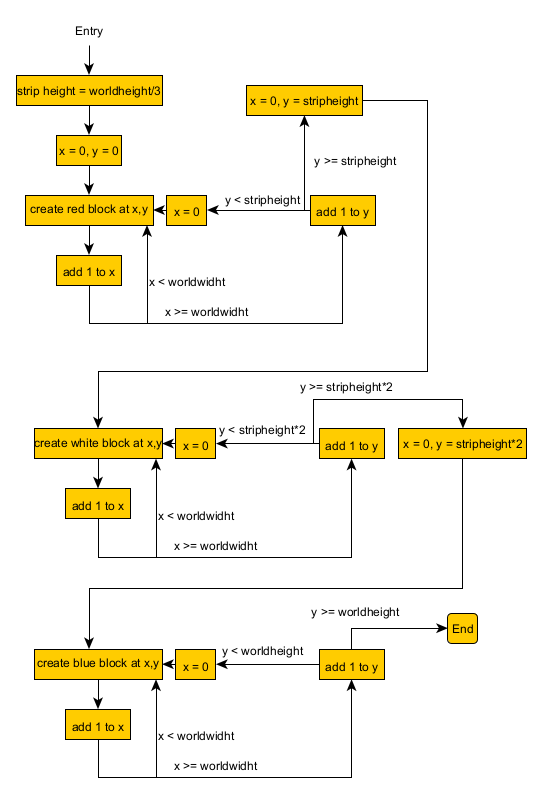
\includegraphics[width=\textwidth]{../flowchart/generateEmptyWorld.png}}
\begin{lstlisting}
function generateEmptyWorld()

Set 2d array world = new int[NEW_WORLD_WIDTH][NEW_WORLD_HEIGHT]
Set redBlock = 1
Set whiteBlock = 4
Set blueBlock = 3
Set stripHeight = NEW_WORLD_HEIGHT / 3

FOR y = 0; y < stripHeight; y++:
    FOR x = 0; x < NEW_WORLD_WIDTH; x++:
        world[x][y] = redBlock

FOR y = stripHeight; y < stripHeight * 2; y++:
    FOR x = 0; x < NEW_WORLD_WIDTH; x++:
        world[x][y] = whiteBlock

FOR y = stripHeight * 2; y < NEW_WORLD_HEIGHT; y++:
    FOR x = 0; x < NEW_WORLD_WIDTH; x++:
        world[x][y] = blueBlock
end function
\end{lstlisting}
\newpage
{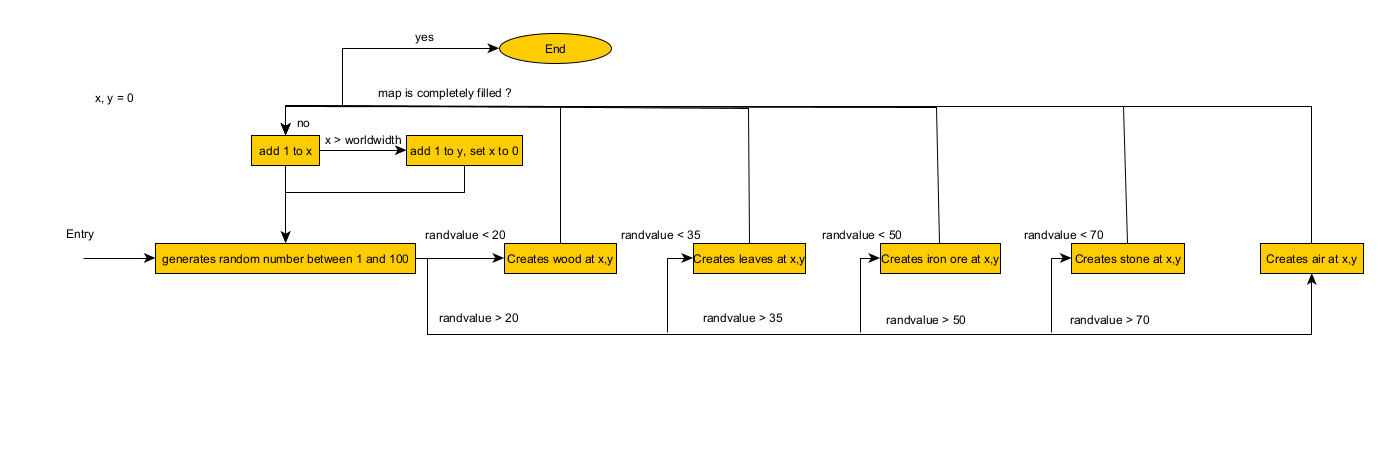
\includegraphics[width=\textwidth]{../flowchart/generateWorld.png}}
\begin{lstlisting}
function generateWorld()

FOR y = 0; y < WORLD_HEIGHT; y++:
  FOR x = 0; x < WORLD_WIDTH; x++:
    creates random number between 1 and 100
    if random number < 20
      creates wood at x, y
    else if random number < 35
      creates leaves at x, y
    else if random number < 50
      creates stone at x, y
    else if random number < 20
      creates iron ore at x, y
   else create air at x, y
end function
\end{lstlisting}
\newpage
{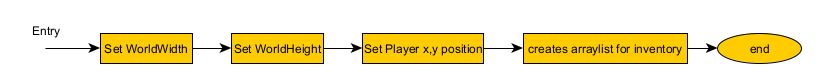
\includegraphics[width=\textwidth]{../flowchart/initGame.png}}
\begin{lstlisting}
function initGame()

Set worldwidth
Set worldheight
Set world = [worldwidht][worldheight]
Set playerx = worldwidght / 2
Set playery = worldheight / 2
Creates array list inventory

\end{lstlisting}
\newpage
{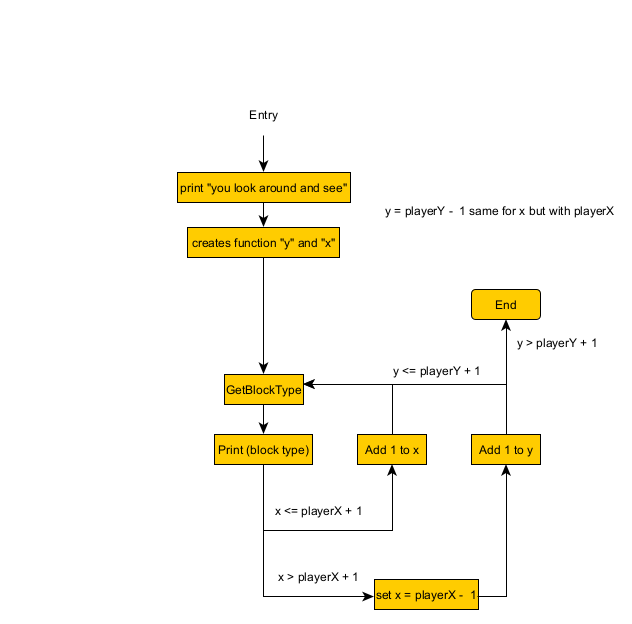
\includegraphics[width=\textwidth]{../flowchart/lookAround.png}}
\begin{lstlisting}
function lookAround()
Set playerX be x position of player
Set playerY be y position of player

print("You look around and see:")
FOR y = Math.max(0, playerY - 1); y <= Math.min(playerY + 1, worldHeight - 1); y++:
  FOR x = Math.max(0, playerX - 1); x <= Math.min(playerX + 1, worldWidth - 1); x++:
    if x == playerX and y == playerY:
      print("P");
    else:
      print(block at position [x][y])
  print empty line
print empty line
end function
\end{lstlisting}
\newpage

{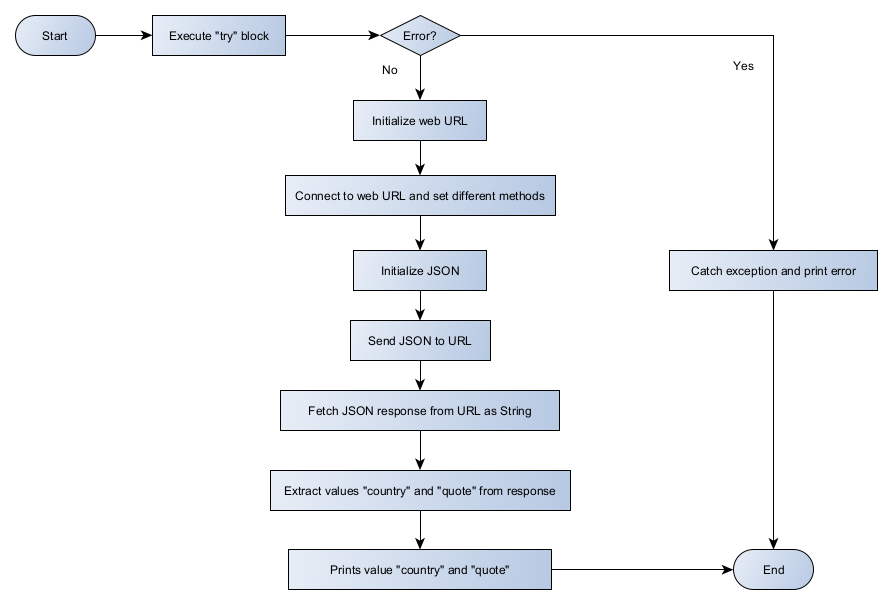
\includegraphics[width=\textwidth]{../flowchart/getCountryAndQuoteFromServer.png}}

\begin{lstlisting}
  function getCountryAndQuoteFromServer():
  TRY:
  Set link = "https://flag.ashish.nl/get_flag"
  Setup a connection to link
  Set request method of connection to "POST"
  Set request property of connection to "Content-Type" as json
  Enable output of connection
  
  let payload be stringified json
  let writer be OutputStreamWriter of connection
        Write payload to writer
        Flush writer
        Close writer
        
        let reader be BufferedReader of connection
        let sb be StringBuilder
        let line be empty string
        WHILE (line is not null):
        let line read next line of reader
        Append line line to sb
            json = ConvertToString(sb)
            
            let countryStart = FindSubstringIndex(json, " ") + 11
            let countryEnd = FindSubstringIndex(json, " ", countryStart)
            let country = Substring(json, countryStart, countryEnd)
            
        let quoteStart = FindSubstringIndex(json, " ") + 9
        let quoteEnd = FindSubstringIndex(json, " ", quoteStart)
        let quote = Substring(json, quoteStart, quoteEnd)
        
        quote = ReplaceSpaces(quote)
        Print("Country: " + country)
        Print("Quote: " + quote)
        CATCH Exception AS e:
        stackTrace = GetStackTrace(e)
        Print("Error connecting to the server")
        Print(stackTrace)
        end function
\end{lstlisting}

{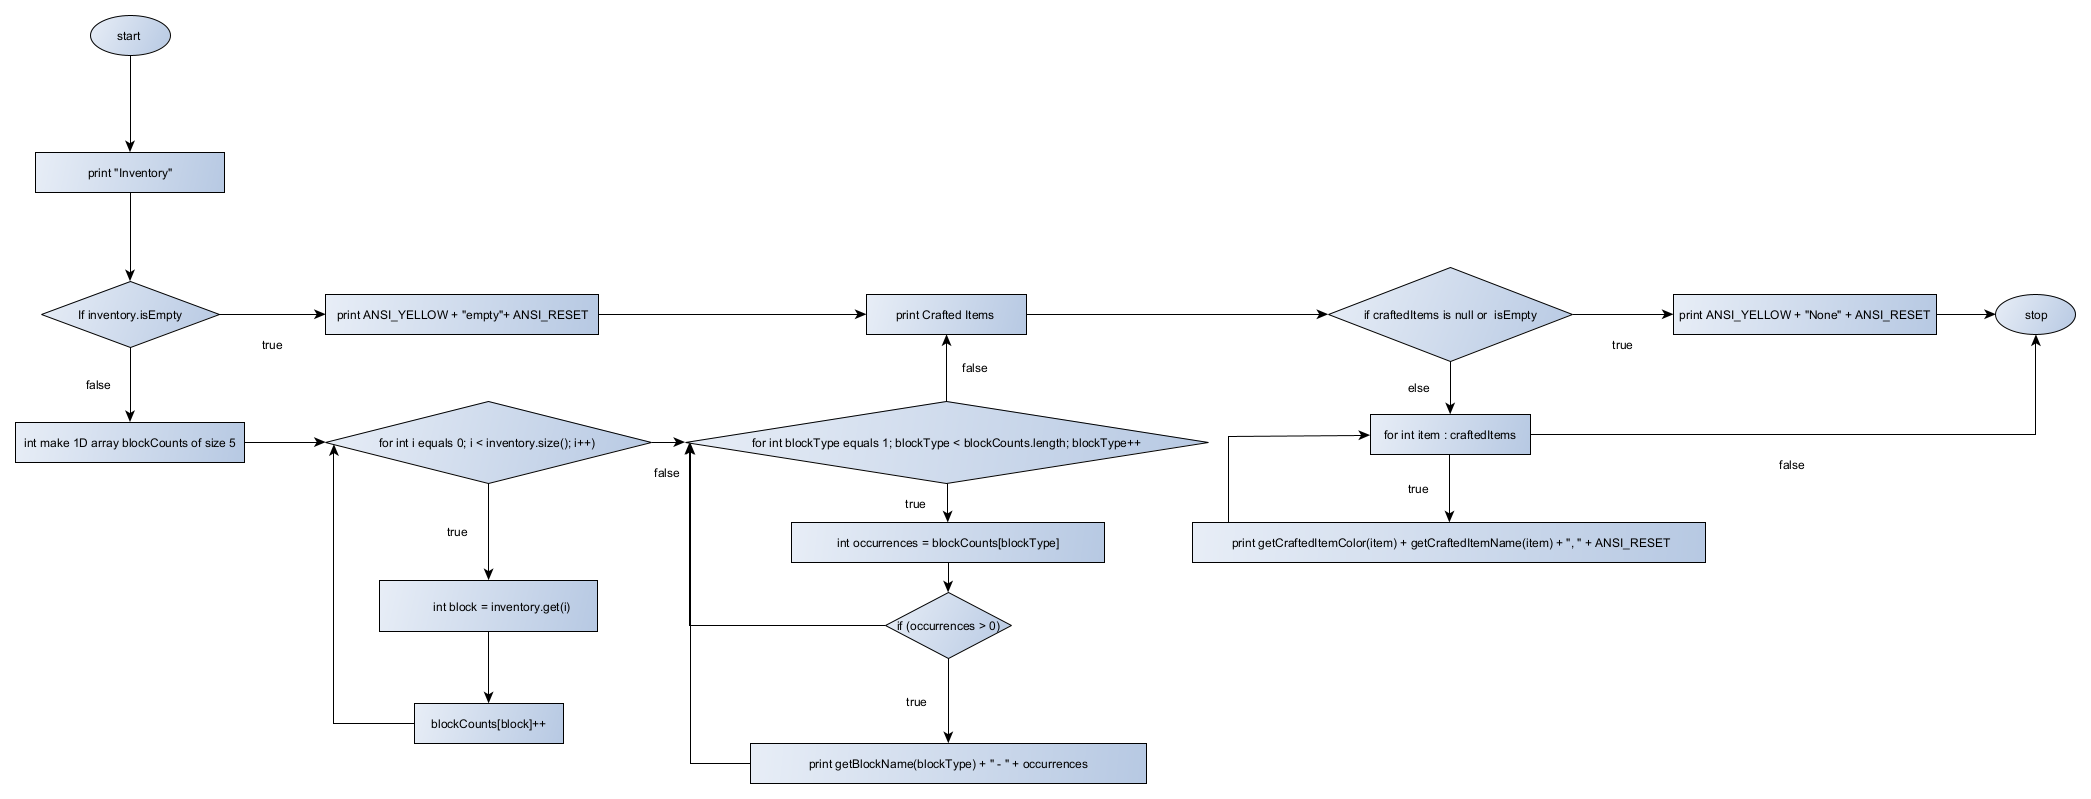
\includegraphics[width=\textwidth]{../flowchart/displayInventory.png}}
\begin{lstlisting}
  function displayInventory:

 print "Inventory"
 if inventory.isEmpty
    print ANSI_YELLOW + " empty" + ANSI_RESET 

else:
   make a 1D array blockCounts of size 5 
   for int i = 0; i < inventory.size(); i++
   int block = inventory.get(i) 
   blockCounts[block] 

For int blockType = 1; blockType < blockCounts.length; blockType++ 
   int occurrences = blockCounts[blockType] 
If occurrences > 0: 
   Print getBlockName(blockType) + " - " + occurrences
print "Crafted Item"
if craftedItems is null or craftedItems is empty
   print ANSI_YELLOW_ + "none" + ANSi_RESET
else 
   for int item : crafted item 
   print getCraftedItemColor(item) + getCraftedItemName(item) + ", " + ANSI_RESET

\end{lstlisting}

{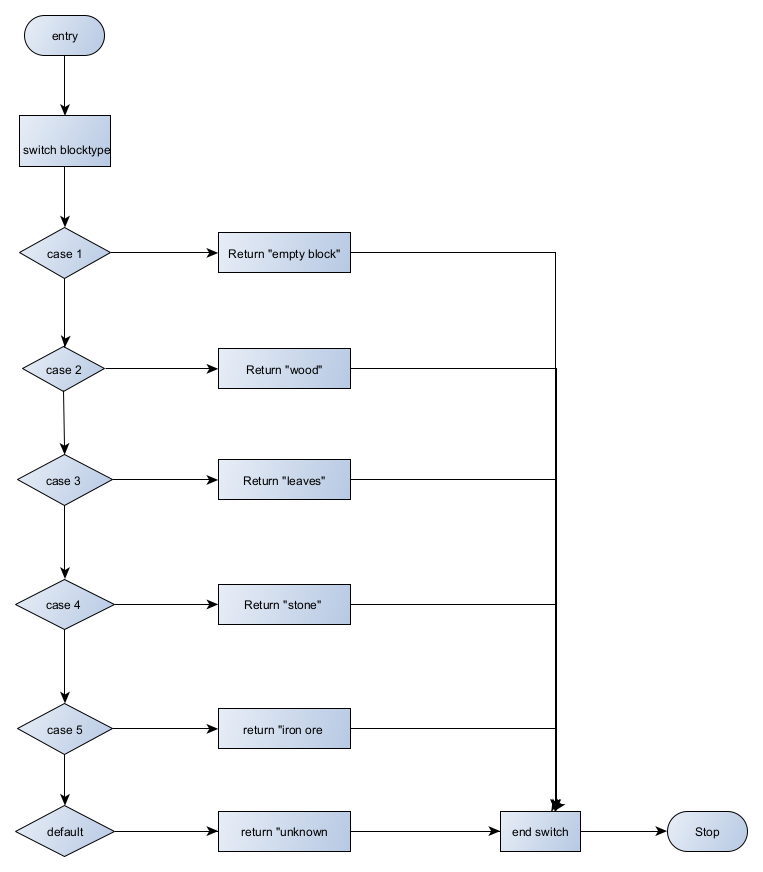
\includegraphics[width=\textwidth]{../flowchart/getBlockName.png}}

\begin{lstlisting}
Function getBlockName(blockType):

Switch blockType 
Case AIR:
 Return "Empty Block" 
Case WOOD: 
Return "Wood" 
Case LEAVES: 
Return "Leaves" 
Case STONE: 
Return "Stone"
 Case IRON_ORE: 
Return "Iron Ore" 
Default:
 Return "Unknown" 

\end{lstlisting}

{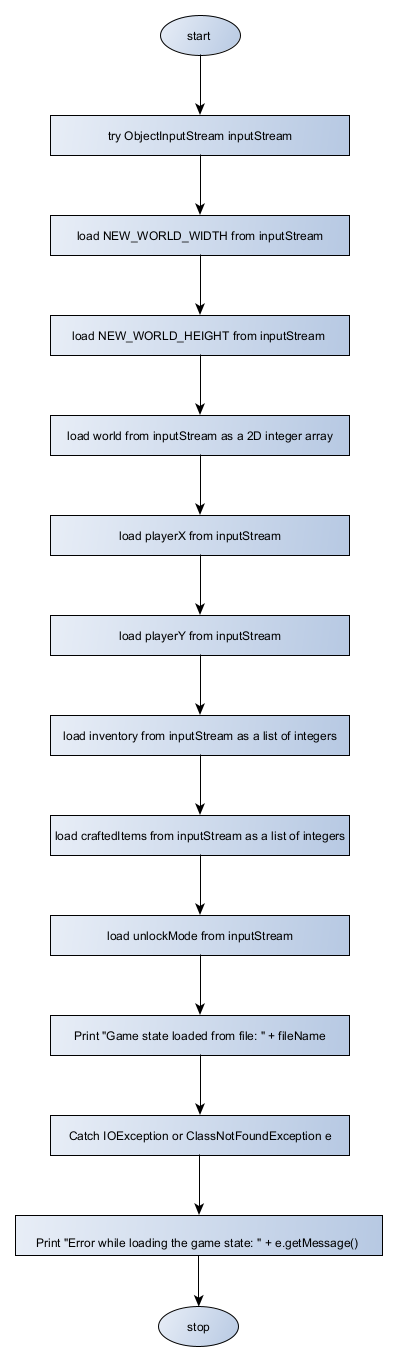
\includegraphics[height=\textheight]{../flowchart/loadGame.png}}

\begin{lstlisting}
  Function loadGame(fileName) 
Try Create ObjectInputStream inputStream using FileInputStream(fileName) 
load NEW_WORLD_WIDTH from inputStream 
load NEW_WORLD_HEIGHT from inputStream 
load world from inputStream as a 2D integer array 
load playerX from inputStream 
load playerY from inputStream 
load inventory from inputStream as a list of integers 
load craftedItems from inputStream as a list of integers 
load unlockMode from inputStream 
Print "Game state loaded from file: " + fileName
 Catch IOException or ClassNotFoundException e 
Print "Error while loading the game state: " + e.getMessage() 

\end{lstlisting}
{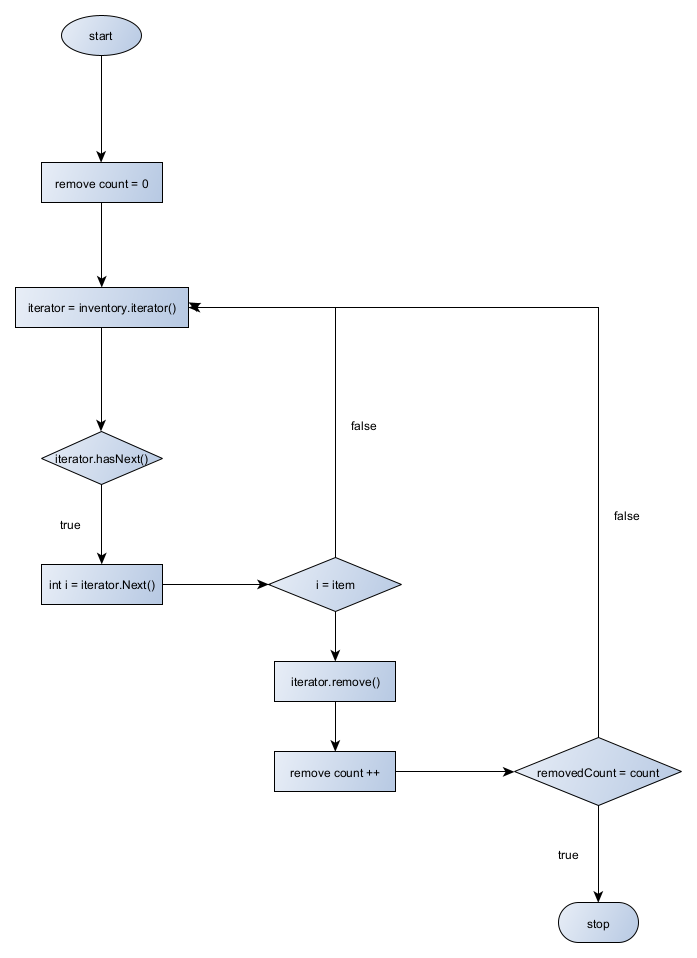
\includegraphics[width=\textwidth]{../flowchart/removeItemsFromInventory.png}}
\begin{lstlisting}
function removeItemsFromInventory(item, count):

removedCount = 0 
iterator = createIterator(inventory) 
While iterator.hasNext()
    i = iterator.next() 
If i is equal to item iterator.remove() 
   removedCount = removedCount + 1 
If removedCount is equal to count
    break
\end{lstlisting}

{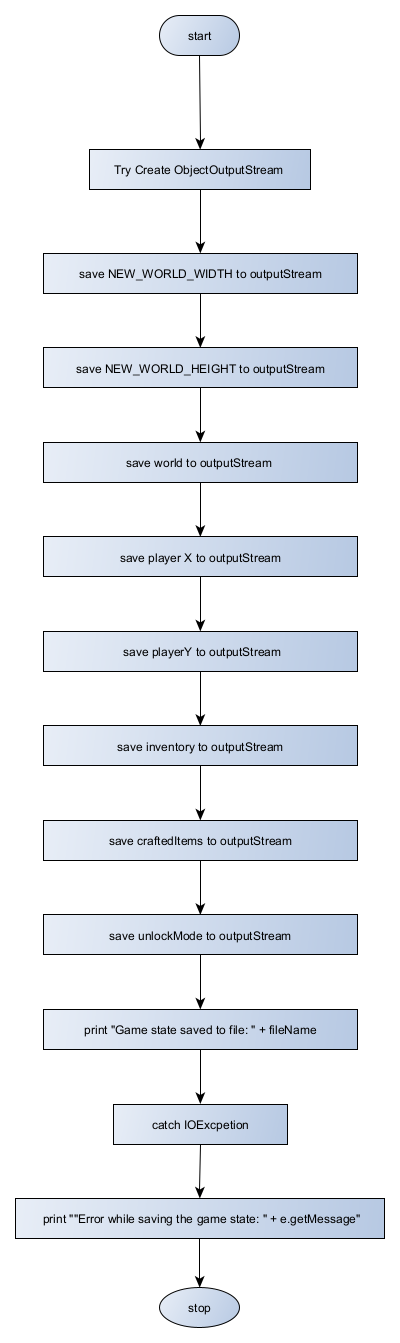
\includegraphics[height=\textheight]{../flowchart/saveGame.png}}

\begin{lstlisting}
  function saveGame(fileName):

Try  ObjectOutputStream outputStream
 save NEW_WORLD_WIDTH to outputStream 
save NEW_WORLD_HEIGHT to outputStream
 save world to outputStream 
save playerX to outputStream
 save playerY to outputStream
 save inventory to outputStream 
save craftedItems to outputStream 
save unlockMode to outputStream
 Print "Game state saved to file: " + fileName Catch IOException e 
Print "Error while saving the game state: " + e.getMessage() 

\end{lstlisting}

